\documentclass[11pt,a4paper]{article}

% ============================================================
% PACKAGES
% ============================================================
\usepackage[a4paper,margin=1in]{geometry}
\usepackage{fancyhdr}
\usepackage{titlesec}
\usepackage[hidelinks,colorlinks=true,linkcolor=black,citecolor=black,urlcolor=blue]{hyperref}
\usepackage{xcolor}
\usepackage{listings}
\usepackage{tikz}
\usepackage{longtable}
\usepackage{booktabs}
\usepackage{array}
\usepackage{float}
\usepackage{multirow}
\usepackage{caption}
\usepackage{amsmath}
\usepackage{setspace}
\usepackage{lastpage}
\usepackage{tabularx}

\usetikzlibrary{shapes,arrows.meta,positioning,fit,backgrounds,calc,decorations.pathreplacing,shadows,trees}

% ============================================================
% COLOR PALETTE
% ============================================================
\definecolor{lumaprimary}{HTML}{2F6690}
\definecolor{lumasecondary}{HTML}{16425B}
\definecolor{lumaaccent}{HTML}{FFA630}
\definecolor{lumalight}{HTML}{E8F1F5}
\definecolor{lumagray}{HTML}{5B5B5B}
\definecolor{lumaok}{HTML}{2E8B57}
\definecolor{lumaerr}{HTML}{C0392B}
\definecolor{codebg}{HTML}{F5F5F5}

% ============================================================
% HEADER / FOOTER
% ============================================================
\pagestyle{fancy}
\fancyhf{}
\renewcommand{\headrulewidth}{0.6pt}
\renewcommand{\footrulewidth}{0.4pt}
\fancyhead[L]{\small\textit{Luma -- Simulator Device Database Schema}}
\fancyhead[R]{\small\thepage}
\fancyfoot[C]{\small SCS 3311 -- Mobile Application Design and Development}

\fancypagestyle{plain}{%
  \fancyhf{}
  \fancyhead[L]{\small\textit{Luma -- Simulator Device Database Schema}}
  \fancyhead[R]{\small\thepage}
  \fancyfoot[C]{\small SCS 3311 -- Mobile Application Design and Development}
  \renewcommand{\headrulewidth}{0.6pt}
}

% ============================================================
% SECTION TITLE STYLING
% ============================================================
\titleformat{\section}
  {\normalfont\Large\bfseries\color{lumasecondary}}
  {\thesection}{1em}{}[{\color{lumaprimary}\titlerule[1pt]}]
\titleformat{\subsection}
  {\normalfont\large\bfseries\color{lumaprimary}}
  {\thesubsection}{1em}{}
\titleformat{\subsubsection}
  {\normalfont\normalsize\bfseries\color{lumasecondary}}
  {\thesubsubsection}{1em}{}

% ============================================================
% TIKZ NODE STYLES
% ============================================================
\tikzset{
  dbnode/.style={rectangle, rounded corners=4pt, draw=lumasecondary, thick,
                 fill=lumaprimary!15, text=lumasecondary, align=center,
                 font=\bfseries, minimum height=0.9cm, inner sep=6pt},
  block/.style={rectangle, rounded corners=3pt, draw=lumagray, thin,
                fill=lumalight!60, text=lumasecondary, align=center,
                font=\scriptsize\bfseries, inner sep=4pt},
  field/.style={rectangle, rounded corners=2pt, draw=lumagray!60, very thin,
                fill=white, text=lumagray, align=center, font=\ttfamily\footnotesize},
  arrow/.style={-{Latex[length=2.5mm]}, thick, color=lumasecondary},
}

% ============================================================
% LISTINGS STYLE
% ============================================================
\lstdefinestyle{codestyle}{
    backgroundcolor=\color{codebg},
    commentstyle=\color{lumagray}\itshape,
    keywordstyle=\color{lumasecondary}\bfseries,
    numberstyle=\tiny\color{lumagray},
    stringstyle=\color{lumaok},
    basicstyle=\ttfamily\footnotesize,
    breakatwhitespace=false,
    breaklines=true,
    captionpos=b,
    keepspaces=true,
    numbers=left,
    numbersep=6pt,
    showspaces=false,
    showstringspaces=false,
    showtabs=false,
    tabsize=2,
    frame=single,
    rulecolor=\color{lumagray!40}
}
\lstset{style=codestyle}

\lstdefinelanguage{json}{
    basicstyle=\ttfamily\footnotesize,
    showstringspaces=false,
    breaklines=true,
    frame=single,
    rulecolor=\color{lumagray!40},
    backgroundcolor=\color{codebg},
    literate=
     *{0}{{{\color{lumaok}0}}}{1}
      {1}{{{\color{lumaok}1}}}{1}
      {2}{{{\color{lumaok}2}}}{1}
      {3}{{{\color{lumaok}3}}}{1}
      {4}{{{\color{lumaok}4}}}{1}
      {5}{{{\color{lumaok}5}}}{1}
      {6}{{{\color{lumaok}6}}}{1}
      {7}{{{\color{lumaok}7}}}{1}
      {8}{{{\color{lumaok}8}}}{1}
      {9}{{{\color{lumaok}9}}}{1}
      {:}{{{\color{lumasecondary}{:}}}}{1}
      {,}{{{\color{lumasecondary}{,}}}}{1}
      {\{}{{{\color{lumasecondary}{\{}}}}{1}
      {\}}{{{\color{lumasecondary}{\}}}}}{1}
      {[}{{{\color{lumasecondary}{[}}}}{1}
      {]}{{{\color{lumasecondary}{]}}}}{1}
}

% ============================================================
% TITLE
% ============================================================
\title{\vspace{-1.5em}\textbf{\color{lumasecondary}Luma -- Hardware Simulator\\ Realtime Database Schema}\vspace{0.4em}}
\author{\small SCS 3311 -- Mobile Application Design and Development}
\date{\small\today}

\begin{document}

\maketitle
\vspace{-2.5em}

% ============================================================
\section{Overview}
\label{sec:overview}

Luma's backend is a single Firebase Realtime Database organized as one JSON tree.
The top-level nodes used by the Hardware Simulator are \texttt{users}, \texttt{devices},
\texttt{alerts}, \texttt{reports}, and \texttt{userLogs}. Floors and rooms are nested under
\texttt{users/\{uid\}}, while device \emph{records} live flat under \texttt{devices} and are
referenced by ID from within the floor/room structure. This deliberate denormalization follows
Firebase's recommended practice of flattening deeply nested data so that listening to a single
device downloads only that device's record rather than an entire room or floor subtree.

\begin{figure}[H]
\centering
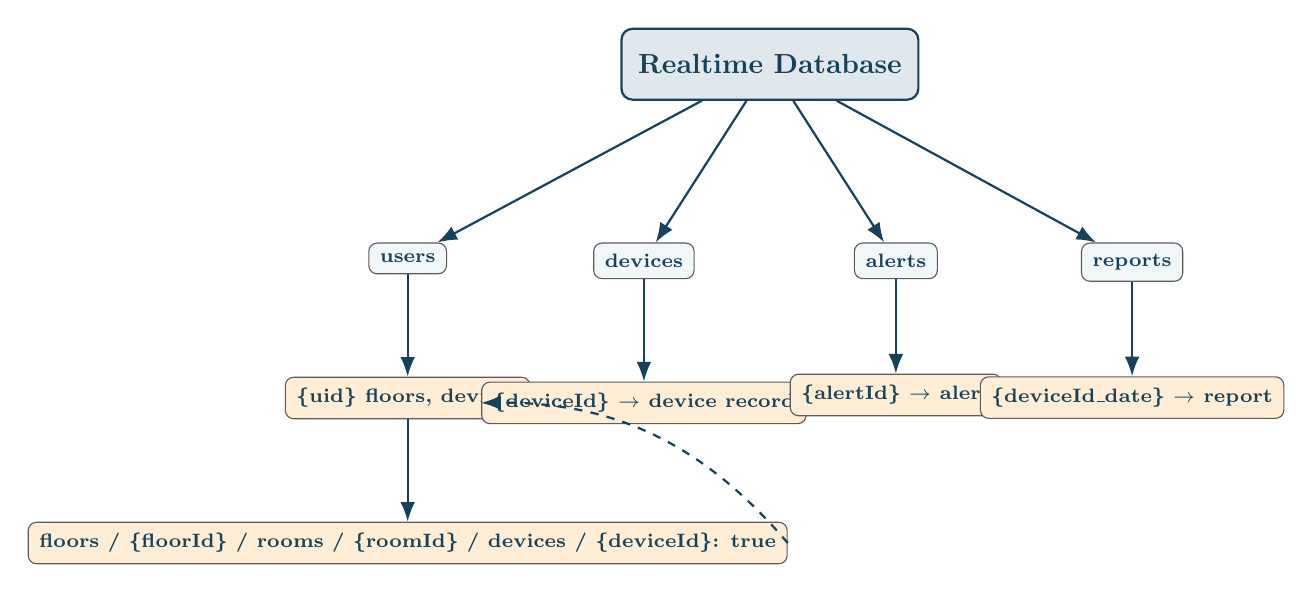
\begin{tikzpicture}[node distance=1.2cm and 2.9cm]
\node[dbnode] (root) {Realtime Database};
\node[block, below=1.8cm of root, xshift=-4.6cm] (users) {users};
\node[block, below=1.8cm of root, xshift=-1.6cm] (devices) {devices};
\node[block, below=1.8cm of root, xshift=1.6cm] (alerts) {alerts};
\node[block, below=1.8cm of root, xshift=4.6cm] (reports) {reports};

\draw[arrow] (root) -- (users);
\draw[arrow] (root) -- (devices);
\draw[arrow] (root) -- (alerts);
\draw[arrow] (root) -- (reports);

\node[block, below=1.3cm of users, fill=lumaaccent!20] (uid) {\{uid\} floors, devices};
\node[block, below=1.3cm of uid, fill=lumaaccent!20] (floors) {floors / \{floorId\} / rooms / \{roomId\} / devices / \{deviceId\}: true};
\draw[arrow] (users) -- (uid);
\draw[arrow] (uid) -- (floors);

\node[block, below=1.3cm of devices, fill=lumaaccent!20] (drec) {\{deviceId\} $\rightarrow$ device record};
\node[block, below=1.2cm of alerts, fill=lumaaccent!20] (arec) {\{alertId\} $\rightarrow$ alert};
\node[block, below=1.2cm of reports, fill=lumaaccent!20] (rrec) {\{deviceId\_date\} $\rightarrow$ report};
\draw[arrow] (devices) -- (drec);
\draw[arrow] (alerts) -- (arec);
\draw[arrow] (reports) -- (rrec);

\draw[-{Latex[length=2.5mm]}, thick, lumasecondary, dashed] (floors.east) to[bend right=25] (drec.west);
\end{tikzpicture}
\caption{Top-level database structure. The dashed arrow indicates a device-ID reference rather than nested ownership.}
\label{fig:schema-overview}
\end{figure}

% ============================================================
\section{The \texttt{devices} Node}
\label{sec:devices}

Each simulated device is stored at \texttt{devices/\{deviceId\}}. A device ID is auto-generated by
the Simulator using the pattern \texttt{device-<timestamp>-<random>} and a new record is created by
\texttt{addDevice()} in \texttt{deviceService.ts}. The record is written into the database with the
following structure, where \texttt{\{...typeFields\}} varies by device type:

\begin{lstlisting}[language=json,caption={Generic shape of a device record.},label={lst:device-generic}]
"devices": {
  "device001": {
    "type": "<type>",
    "name": "Living Room Light",
    "state": "ON | OFF",
    "status": "ON | OFF | ONLINE | ERROR | DISCONNECTED",
    "lastSeen": 1739000000000,
    "userId": "UID",
    "...typeFields": { }
  }
}
\end{lstlisting}

\subsection{Common Fields}
\label{sub:common}

Table~\ref{tab:common-fields} lists the fields shared by all five device types
(\texttt{outlet}, \texttt{light}, \texttt{iron}, \texttt{switchPanel}, \texttt{camera}).

\begin{table}[H]
\centering
\caption{Fields common to every device record.}
\label{tab:common-fields}
\begin{tabularx}{\textwidth}{@{}l l X X@{}}
\toprule
\textbf{Field} & \textbf{Type} & \textbf{Values / Units} & \textbf{Description} \\
\midrule
\texttt{type} & string & \texttt{outlet}, \texttt{light}, \texttt{iron}, \texttt{switchPanel}, \texttt{camera} & Discriminator that selects the device-specific fields and controls. \\
\texttt{name} & string & free text & Human-readable device name shown in both clients. \\
\texttt{state} & string & \texttt{ON} / \texttt{OFF} & Power state written by the on/off control. Absent for cameras (which are always ``streaming''). \\
\texttt{status} & string & \texttt{ON} / \texttt{OFF} / \texttt{ONLINE} / \texttt{ERROR} / \texttt{DISCONNECTED} & Connectivity/health status; cameras default to \texttt{ONLINE}. \\
\texttt{lastSeen} & number & epoch ms & Heartbeat timestamp; written on every state change. Consumed by the disconnection-detector Cloud Function. \\
\texttt{userId} & string & Firebase UID & Owning user; used to scope the per-user device index. \\
\bottomrule
\end{tabularx}
\end{table}

\subsection{Type-Specific Fields}
\label{sub:typefields}

The tables below list the extra fields written for each device type, as produced by
\texttt{AddDeviceDialog.tsx} and consumed by the Cloud Functions.

\subsubsection{Electrical Outlet (\texttt{outlet})}
An outlet has no extra fields beyond the common ones; it is the baseline ON/OFF device.

\subsubsection{Smart Light (\texttt{light})}
\begin{table}[H]
\centering
\caption{Fields specific to \texttt{light} devices.}
\begin{tabularx}{\textwidth}{@{}l l X X@{}}
\toprule
\textbf{Field} & \textbf{Type} & \textbf{Values / Units} & \textbf{Description} \\
\midrule
\texttt{startTime} & string & \texttt{"HH:MM"} & Automatic on time, consumed by the light-scheduler Cloud Function. \\
\texttt{endTime} & string & \texttt{"HH:MM"} & Automatic off time, consumed by the light-scheduler Cloud Function. \\
\texttt{turnedOnAt} & number | null & epoch ms & Set to \texttt{Date.now()} when turned on; cleared on off/shutdown. \\
\bottomrule
\end{tabularx}
\end{table}

\subsubsection{Electric Iron (\texttt{iron})}
\begin{table}[H]
\centering
\caption{Fields specific to \texttt{iron} devices.}
\begin{tabularx}{\textwidth}{@{}l l X X@{}}
\toprule
\textbf{Field} & \textbf{Type} & \textbf{Values / Units} & \textbf{Description} \\
\midrule
\texttt{turnedOnAt} & number | null & epoch ms & Time the iron was switched on; used to measure elapsed run time. \\
\texttt{maxDurationMinutes} & number & 5--120 (step 5, default 30) & Safety auto-shutdown limit enforced by the iron auto-shutdown Cloud Function. \\
\bottomrule
\end{tabularx}
\end{table}

\subsubsection{Multi-Switch Panel (\texttt{switchPanel})}
\begin{table}[H]
\centering
\caption{Fields specific to \texttt{switchPanel} devices.}
\begin{tabularx}{\textwidth}{@{}l l X X@{}}
\toprule
\textbf{Field} & \textbf{Type} & \textbf{Values / Units} & \textbf{Description} \\
\midrule
\texttt{switchCount} & number & 2--5 (default 3) & Number of physical switches on the panel. \\
\texttt{switches} & object & \texttt{\{switch1: "ON|OFF", ...\}} & One key per switch (\texttt{switch1}\dots\texttt{switchN}); each toggled independently via \texttt{setSwitchState()}. \\
\bottomrule
\end{tabularx}
\end{table}

\subsubsection{Camera (\texttt{camera})}
\begin{table}[H]
\centering
\caption{Fields specific to \texttt{camera} devices.}
\begin{tabularx}{\textwidth}{@{}l l X X@{}}
\toprule
\textbf{Field} & \textbf{Type} & \textbf{Values / Units} & \textbf{Description} \\
\midrule
\texttt{lastSnapshotUrl} & string & HTTPS URL & Most recent mock image URL (generated via \texttt{picsum.photos}). \\
\texttt{lastSnapshotImage} & string & base64 data URL & base64-encoded JPEG of the snapshot stored so mobile clients can render the same feed without resolving an external URL. \\
\texttt{lastSnapshotAt} & number & epoch ms & Time the snapshot was requested. \\
\bottomrule
\end{tabularx}
\end{table}

\subsubsection{Power Usage History (\texttt{history})}
Written by the report-aggregator Cloud Function when a device transitions \texttt{ON} $\rightarrow$ \texttt{OFF}.
Each entry is pushed onto \texttt{devices/\{deviceId\}/history}:

\begin{table}[H]
\centering
\caption{Fields of each \texttt{history} entry.}
\begin{tabularx}{\textwidth}{@{}l l X X@{}}
\toprule
\textbf{Field} & \textbf{Type} & \textbf{Values / Units} & \textbf{Description} \\
\midrule
\texttt{turnedOffAt} & number & epoch ms & When the device was switched off. \\
\texttt{durationMinutes} & number & minutes & Length of the on-session, rounded to the nearest minute. \\
\texttt{estimatedKwh} & number & kWh (3 d.p.) & Estimated energy consumed, computed from nominal wattage \texttimes\ duration. \\
\bottomrule
\end{tabularx}
\end{table}

% ============================================================
\section{The \texttt{users} Node}
\label{sec:users}

Floors, rooms, and a per-user device index live under \texttt{users/\{uid\}}. Room membership is
expressed as a set of device-ID references (\texttt{\{deviceId\}: true}); the device records
themselves remain in the flat \texttt{devices} node.

\begin{table}[H]
\centering
\caption{Structure of the \texttt{users} node.}
\label{tab:users}
\begin{tabularx}{\textwidth}{@{}l l X X@{}}
\toprule
\textbf{Path} & \textbf{Type} & \textbf{Values} & \textbf{Description} \\
\midrule
\texttt{users/\{uid\}/floors/\{floorId\}/name} & string & free text & Floor display name (e.g.\ ``Ground Floor''). \\
\texttt{users/\{uid\}/floors/\{floorId\}/icon} & string & \texttt{home}, \texttt{stairs}, \texttt{attic}, \ldots & Icon key rendered by the clients. \\
\texttt{users/\{uid\}/floors/\{floorId\}/rooms/\{roomId\}/name} & string & free text & Room display name (e.g.\ ``Living Room''). \\
\texttt{users/\{uid\}/floors/\{floorId\}/rooms/\{roomId\}/devices/\{deviceId\}} & boolean & \texttt{true} & Membership reference to a device record. \\
\texttt{users/\{uid\}/devices/\{deviceId\}} & boolean & \texttt{true} & Flattened index of all devices owned by the user. \\
\bottomrule
\end{tabularx}
\end{table}

% ============================================================
\section{The \texttt{alerts} Node}
\label{sec:alerts}

Alerts are pushed by the Cloud Functions (iron auto-shutdown, disconnection detector) and read by the
Simulator's alert list. Each record is keyed by an auto-generated push ID.

\begin{table}[H]
\centering
\caption{Fields of an \texttt{alerts} record.}
\label{tab:alerts}
\begin{tabularx}{\textwidth}{@{}l l X X@{}}
\toprule
\textbf{Field} & \textbf{Type} & \textbf{Values / Units} & \textbf{Description} \\
\midrule
\texttt{deviceId} & string & device ID & The device the alert concerns. \\
\texttt{type} & string & \texttt{AUTO\_SHUTDOWN}, \texttt{DEVICE\_DISCONNECTED} & Machine-readable alert category. \\
\texttt{message} & string & free text & Human-readable alert description. \\
\texttt{timestamp} & number & epoch ms & When the alert was raised. \\
\bottomrule
\end{tabularx}
\end{table}

% ============================================================
\section{The \texttt{reports} Node}
\label{sec:reports}

Usage reports are written exclusively by the report-aggregator Cloud Function (client writes are
denied by the security rules). Each record is keyed \texttt{\{deviceId\}\_\{YYYY-MM-DD\}} and
aggregates a device's sessions for the day, week, and month.

\begin{table}[H]
\centering
\caption{Fields of a \texttt{reports} record.}
\label{tab:reports}
\begin{tabularx}{\textwidth}{@{}l l X X@{}}
\toprule
\textbf{Field} & \textbf{Type} & \textbf{Values / Units} & \textbf{Description} \\
\midrule
\texttt{deviceId} & string & device ID & The device this report covers. \\
\texttt{deviceName} & string & free text & Device name snapshot at aggregation time. \\
\texttt{deviceType} & string & one of the five types & Device type snapshot. \\
\texttt{period} & string & \texttt{daily} & Reporting period of the record. \\
\texttt{date} & string & \texttt{YYYY-MM-DD} & Day the record covers. \\
\texttt{week} & string & \texttt{YYYY-MM-DD} (week start) & Week the record contributes to. \\
\texttt{month} & string & \texttt{YYYY-MM} & Month the record contributes to. \\
\texttt{totalOnDurationMinutes} & number & minutes & Cumulative on-duration for the day. \\
\texttt{totalSessions} & number & count & Number of on/off sessions recorded. \\
\texttt{estimatedKwh} & number & kWh (3 d.p.) & Cumulative estimated energy usage. \\
\texttt{lastUpdated} & number & epoch ms & Last time the report was recomputed. \\
\bottomrule
\end{tabularx}
\end{table}

% ============================================================
\section{The \texttt{userLogs} Node}
\label{sec:userlogs}

The Simulator records a usage/audit log for each signed-in user. Every entry is pushed onto
\texttt{userLogs/\{uid\}} by the \texttt{logEvent()} callback in \texttt{App.tsx}.

\begin{table}[H]
\centering
\caption{Fields of a \texttt{userLogs} entry.}
\label{tab:userlogs}
\begin{tabularx}{\textwidth}{@{}l l X X@{}}
\toprule
\textbf{Field} & \textbf{Type} & \textbf{Values / Units} & \textbf{Description} \\
\midrule
\texttt{environment} & string & \texttt{simulator} & Client that produced the log entry. \\
\texttt{device} & string & user agent string & Browser/platform of the client. \\
\texttt{event} & string & e.g.\ \texttt{session\_start}, \texttt{device\_toggle} & Event name. \\
\texttt{sessionId} & string & random UUID & Identifies a browser session. \\
\texttt{timestamp} & number & epoch ms & When the event occurred. \\
\texttt{details} & object & key/value metadata & Per-event context (e.g.\ \texttt{\{deviceId, state\}}). \\
\bottomrule
\end{tabularx}
\end{table}

% ============================================================
\section{Complete JSON Example}
\label{sec:example}

The listing below shows the full tree written by \texttt{seedSampleData()} together with the
alert, report, and log records produced by the Cloud Functions and Simulator.

\begin{lstlisting}[language=json,caption={Complete database tree for the seeded home.},label={lst:schema-full}]
{
  "devices": {
    "device001": {
      "type": "light", "name": "Living Room Light",
      "state": "OFF", "status": "OFF",
      "startTime": "18:00", "endTime": "23:00",
      "turnedOnAt": null,
      "lastSeen": 1739000000000, "userId": "UID"
    },
    "device003": {
      "type": "iron", "name": "Bedroom Iron",
      "state": "OFF", "status": "OFF",
      "turnedOnAt": null, "maxDurationMinutes": 30,
      "lastSeen": 1739000000000, "userId": "UID",
      "history": {
        "-Oabc123": {
          "turnedOffAt": 1739000400000,
          "durationMinutes": 25,
          "estimatedKwh": 0.417
        }
      }
    },
    "device004": {
      "type": "switchPanel", "name": "Study Switch Panel",
      "switchCount": 3,
      "switches": { "switch1": "OFF", "switch2": "OFF", "switch3": "OFF" },
      "status": "OFF",
      "lastSeen": 1739000000000, "userId": "UID"
    },
    "device005": {
      "type": "camera", "name": "Garage Camera",
      "status": "ONLINE",
      "lastSnapshotUrl": "https://picsum.photos/seed/camera-garage/640/480",
      "lastSnapshotImage": "data:image/jpeg;base64,/9j/4AAQSkZJRgABAQAAAQABAAD...",
      "lastSnapshotAt": 1739000000000,
      "lastSeen": 1739000000000, "userId": "UID"
    }
  },
  "users": {
    "UID": {
      "floors": {
        "floor001": {
          "name": "Ground Floor", "icon": "home",
          "rooms": {
            "room001": {
              "name": "Living Room",
              "devices": { "device001": true }
            }
          }
        }
      },
      "devices": { "device001": true, "device003": true }
    }
  },
  "alerts": {
    "-Oxyz789": {
      "deviceId": "device003",
      "type": "AUTO_SHUTDOWN",
      "message": "Iron \"Bedroom Iron\" automatically turned OFF after 30 minutes for safety",
      "timestamp": 1739001800000
    }
  },
  "reports": {
    "device003_2026-07-10": {
      "deviceId": "device003", "deviceName": "Bedroom Iron",
      "deviceType": "iron", "period": "daily",
      "date": "2026-07-10", "week": "2026-07-06", "month": "2026-07",
      "totalOnDurationMinutes": 48, "totalSessions": 2,
      "estimatedKwh": 0.8, "lastUpdated": 1739001800000
    }
  },
  "userLogs": {
    "UID": {
      "-Olog456": {
        "environment": "simulator",
        "device": "Mozilla/5.0 (X11; Linux x86_64) ...",
        "event": "device_toggle",
        "sessionId": "a1b2c3d4",
        "timestamp": 1739001200000,
        "details": { "deviceId": "device001", "state": "ON" }
      }
    }
  }
}
\end{lstlisting}

\end{document}
